% Options for packages loaded elsewhere
\PassOptionsToPackage{unicode}{hyperref}
\PassOptionsToPackage{hyphens}{url}
\PassOptionsToPackage{dvipsnames,svgnames*,x11names*}{xcolor}
%
\documentclass[
  12pt,
]{article}
\usepackage[]{mathpazo}
\usepackage{setspace}
\usepackage{amssymb,amsmath}
\usepackage{ifxetex,ifluatex}
\ifnum 0\ifxetex 1\fi\ifluatex 1\fi=0 % if pdftex
  \usepackage[T1]{fontenc}
  \usepackage[utf8]{inputenc}
  \usepackage{textcomp} % provide euro and other symbols
\else % if luatex or xetex
  \usepackage{unicode-math}
  \defaultfontfeatures{Scale=MatchLowercase}
  \defaultfontfeatures[\rmfamily]{Ligatures=TeX,Scale=1}
\fi
% Use upquote if available, for straight quotes in verbatim environments
\IfFileExists{upquote.sty}{\usepackage{upquote}}{}
\IfFileExists{microtype.sty}{% use microtype if available
  \usepackage[]{microtype}
  \UseMicrotypeSet[protrusion]{basicmath} % disable protrusion for tt fonts
}{}
\makeatletter
\@ifundefined{KOMAClassName}{% if non-KOMA class
  \IfFileExists{parskip.sty}{%
    \usepackage{parskip}
  }{% else
    \setlength{\parindent}{0pt}
    \setlength{\parskip}{6pt plus 2pt minus 1pt}}
}{% if KOMA class
  \KOMAoptions{parskip=half}}
\makeatother
\usepackage{xcolor}
\IfFileExists{xurl.sty}{\usepackage{xurl}}{} % add URL line breaks if available
\IfFileExists{bookmark.sty}{\usepackage{bookmark}}{\usepackage{hyperref}}
\hypersetup{
  colorlinks=true,
  linkcolor=blue,
  filecolor=Maroon,
  citecolor=Blue,
  urlcolor=Blue,
  pdfcreator={LaTeX via pandoc}}
\urlstyle{same} % disable monospaced font for URLs
\usepackage[margin=1in]{geometry}
\usepackage{graphicx}
\makeatletter
\def\maxwidth{\ifdim\Gin@nat@width>\linewidth\linewidth\else\Gin@nat@width\fi}
\def\maxheight{\ifdim\Gin@nat@height>\textheight\textheight\else\Gin@nat@height\fi}
\makeatother
% Scale images if necessary, so that they will not overflow the page
% margins by default, and it is still possible to overwrite the defaults
% using explicit options in \includegraphics[width, height, ...]{}
\setkeys{Gin}{width=\maxwidth,height=\maxheight,keepaspectratio}
% Set default figure placement to htbp
\makeatletter
\def\fps@figure{htbp}
\makeatother
\setlength{\emergencystretch}{3em} % prevent overfull lines
\providecommand{\tightlist}{%
  \setlength{\itemsep}{0pt}\setlength{\parskip}{0pt}}
\setcounter{secnumdepth}{-\maxdimen} % remove section numbering
\usepackage{hyperref}
\usepackage[]{natbib}
\bibliographystyle{plainnat}

\author{}
\date{\vspace{-2.5em}}

\begin{document}

\setstretch{1}
\begin{flushright} 
    \end{flushright}
    \begin{center} \textbf{Parlr: Frequently Asked Questions}
    
    Brian Kundinger

    \end{center}

\hypertarget{what-are-parlrs-competitors}{%
\subsubsection{What are parlr's
competitors?}\label{what-are-parlrs-competitors}}

Most record linkage techniques are derived from the seminal 1969 paper
by Fellegi and Sunter: ``A Theory for Record Linkage''. The defining
characteristic of their model was to transform the sets of records,
which constitute text data that is difficult to model, into sets of
comparison vectors governed by parameters that can be more easily
estimated. Concretely, if files \(A\) and \(B\) have \(n_A\) and \(n_B\)
records respectively, and if the files share \(F\) fields in common upon
which to base the linkage, the Fellegi and Sunter approach generates a
\(n_A n_B \times F\) matrix \(\Gamma\), which contains similarity scores
between each pair of records across datasets. We say \(\gamma_{ij}\) is
the comparison vector for record \(i \in A\) and record \(j \in B\),
with \(\gamma_{ij}^f\) providing their similarity score on the
\(f^{th}\) field. For ease of modeling and computation, we restrict
these similarity scores to be discrete, ordinal variables, and the
construction of these is left to the modeller. With notation
\(\gamma_{ij}^f \in \{0, \ldots, L_f - 1\}\) for the number of possible
agreement levels for field \(f\), we use binary 0-1 variables to
indicate exact matching, and 0-1-2 variables to provide an option for
partial matching. For text data, we calculate similarity based on
Levenstein distance or some other text similarity score, and bin these
scores to integers for use in the model.

Two modern adaptations of the Fellegi Sunter model are important for
understanding \texttt{parlr} and its contribution. In 2019, Enamorado et
al proposed \texttt{fastlink}, a method that closely followed the
modelling assumptions of Fellegi and Sunter, but used innovating hashing
techniques to greatly enhance its speed and scale. Importantly, they
maintained Fellegi and Sunter's independent matching assumption, in
which the matching status of any \((i,j)\) pair is made independently of
the matching of any other \((i', j')\). This leads to many matchings
that violate ``one-to-one'' considerations that are often implicit in
the data, which need to be resolved in a post-processing step. In
contrast, Sadinle (2017) proposed ``Beta Record Linkage for Bipartite
Matching'' and the accompanying \texttt{BRL} package which strictly
enforces one-to-one matching. Specifically, in each iteration of his
Gibbs sampler, he considers each record \(j\in B\), removes from
consideration the records \(i\in A\) that have already been matched,
then samples a potential link. However, accounting for these
dependencies throughout the linkage process is computionally burdensome,
leaving \texttt{BRL} only suitable for small to moderate linkage
problems.

\hypertarget{how-is-parlr-different}{%
\subsubsection{How is parlr different?}\label{how-is-parlr-different}}

While \texttt{fastlink} makes \(n_A \times n_B\) many indepedent binary
linkage decisions and Sadinle makes \(n_B\) many \emph{dependent}
linkage decisions among \(n_A\) many options, \texttt{parlr} strikes
middle ground by making \(n_B\) many \emph{independent} linkage
decisions among \(n_A\) many options. That is, in each iteration of the
Gibbs sampler, we make one linkage decision per \(j \in B\), but do not
remove previously matched records from consideration. While this does
mean that a particular iteration of the Gibbs sampler may contain some
matchings that violate one-to-one requirements, these violations happen
infreqently and randomly across all record pairing, so that they do not
seriously harm the final Bayes estimate of the linkage structure we make
from all the Gibbs samples. In cases where our Bayes estimate does
contain matches that violate one-to-one, we note that such cases far
less frequently than under \texttt{fastlink}, and that these cases are
easily resolved by simply taking the match pair with the highest
posterior match probability.

Broadly speaking, we increase our computational efficiency by
recognizing that record pairs contribute to posterior calculations only
through the agreement pattern of the \(\gamma_{ij}\) vector. Let \(H\)
be the set of unique agreement patterns in the data, let \(P\) denote
the total number of unique agreement patterns. Note that \(P\) is
bounded above by \(\prod_{f=1}^F L_f\), and that this bound does not
scale with \(n_A\) or \(n_B\). We index these agreement patterns by
\(p \in \{1, \ldots, P\}\), and say \((i,j) \in h_p\) when the \((i,j)\)
pair exhibits the \(p^{th}\) agreement pattern. Wherever possible, we
conduct calculations over these \(P\) agreement patterns rather than the
\(n_A \times n_B\) record pairs.

By making linkage decisions for each \(j\in B\) independently, we do not
need to concern ourselves with the precise record label for \(j's\)
potential pairing within the Gibbs sampler, only the agreement pattern
of the \(\gamma\) vector. While the original Fellegi Sunter framework
has computational complexity \(O(n_A \times n_B)\), these modifications
completely remove dependence on \(n_A\) throughout the Gibbs sampler,
reducing the complexity to \(O(n_B)\)

\hypertarget{how-accurate-is-it}{%
\subsubsection{How accurate is it?}\label{how-accurate-is-it}}

In his 2017 paper, Sadinle demonstrated the strength of his method by
running \texttt{BRL} on simulated pairs of files with differing levels
of errors and overlap. Comparing our method against \texttt{BRL} on
these same simulated datasets, we find that our method only has weakend
performance in the extreme scenario of very high errors and very high
overlap across files.
\[\text{Recall} = \frac{\text{Matches Correctly Identified}}{\text{True Matches in Data}}\]
\[\text{Precision} = \frac{\text{Declared Matches}}{\text{True Matches in Data}}\]
\[\text{F-Measure} = 2\left(\frac{\text{Recall} \times \text{Precision}}{\text{Recall} + \text{Precision}}\right)\]

\begin{center}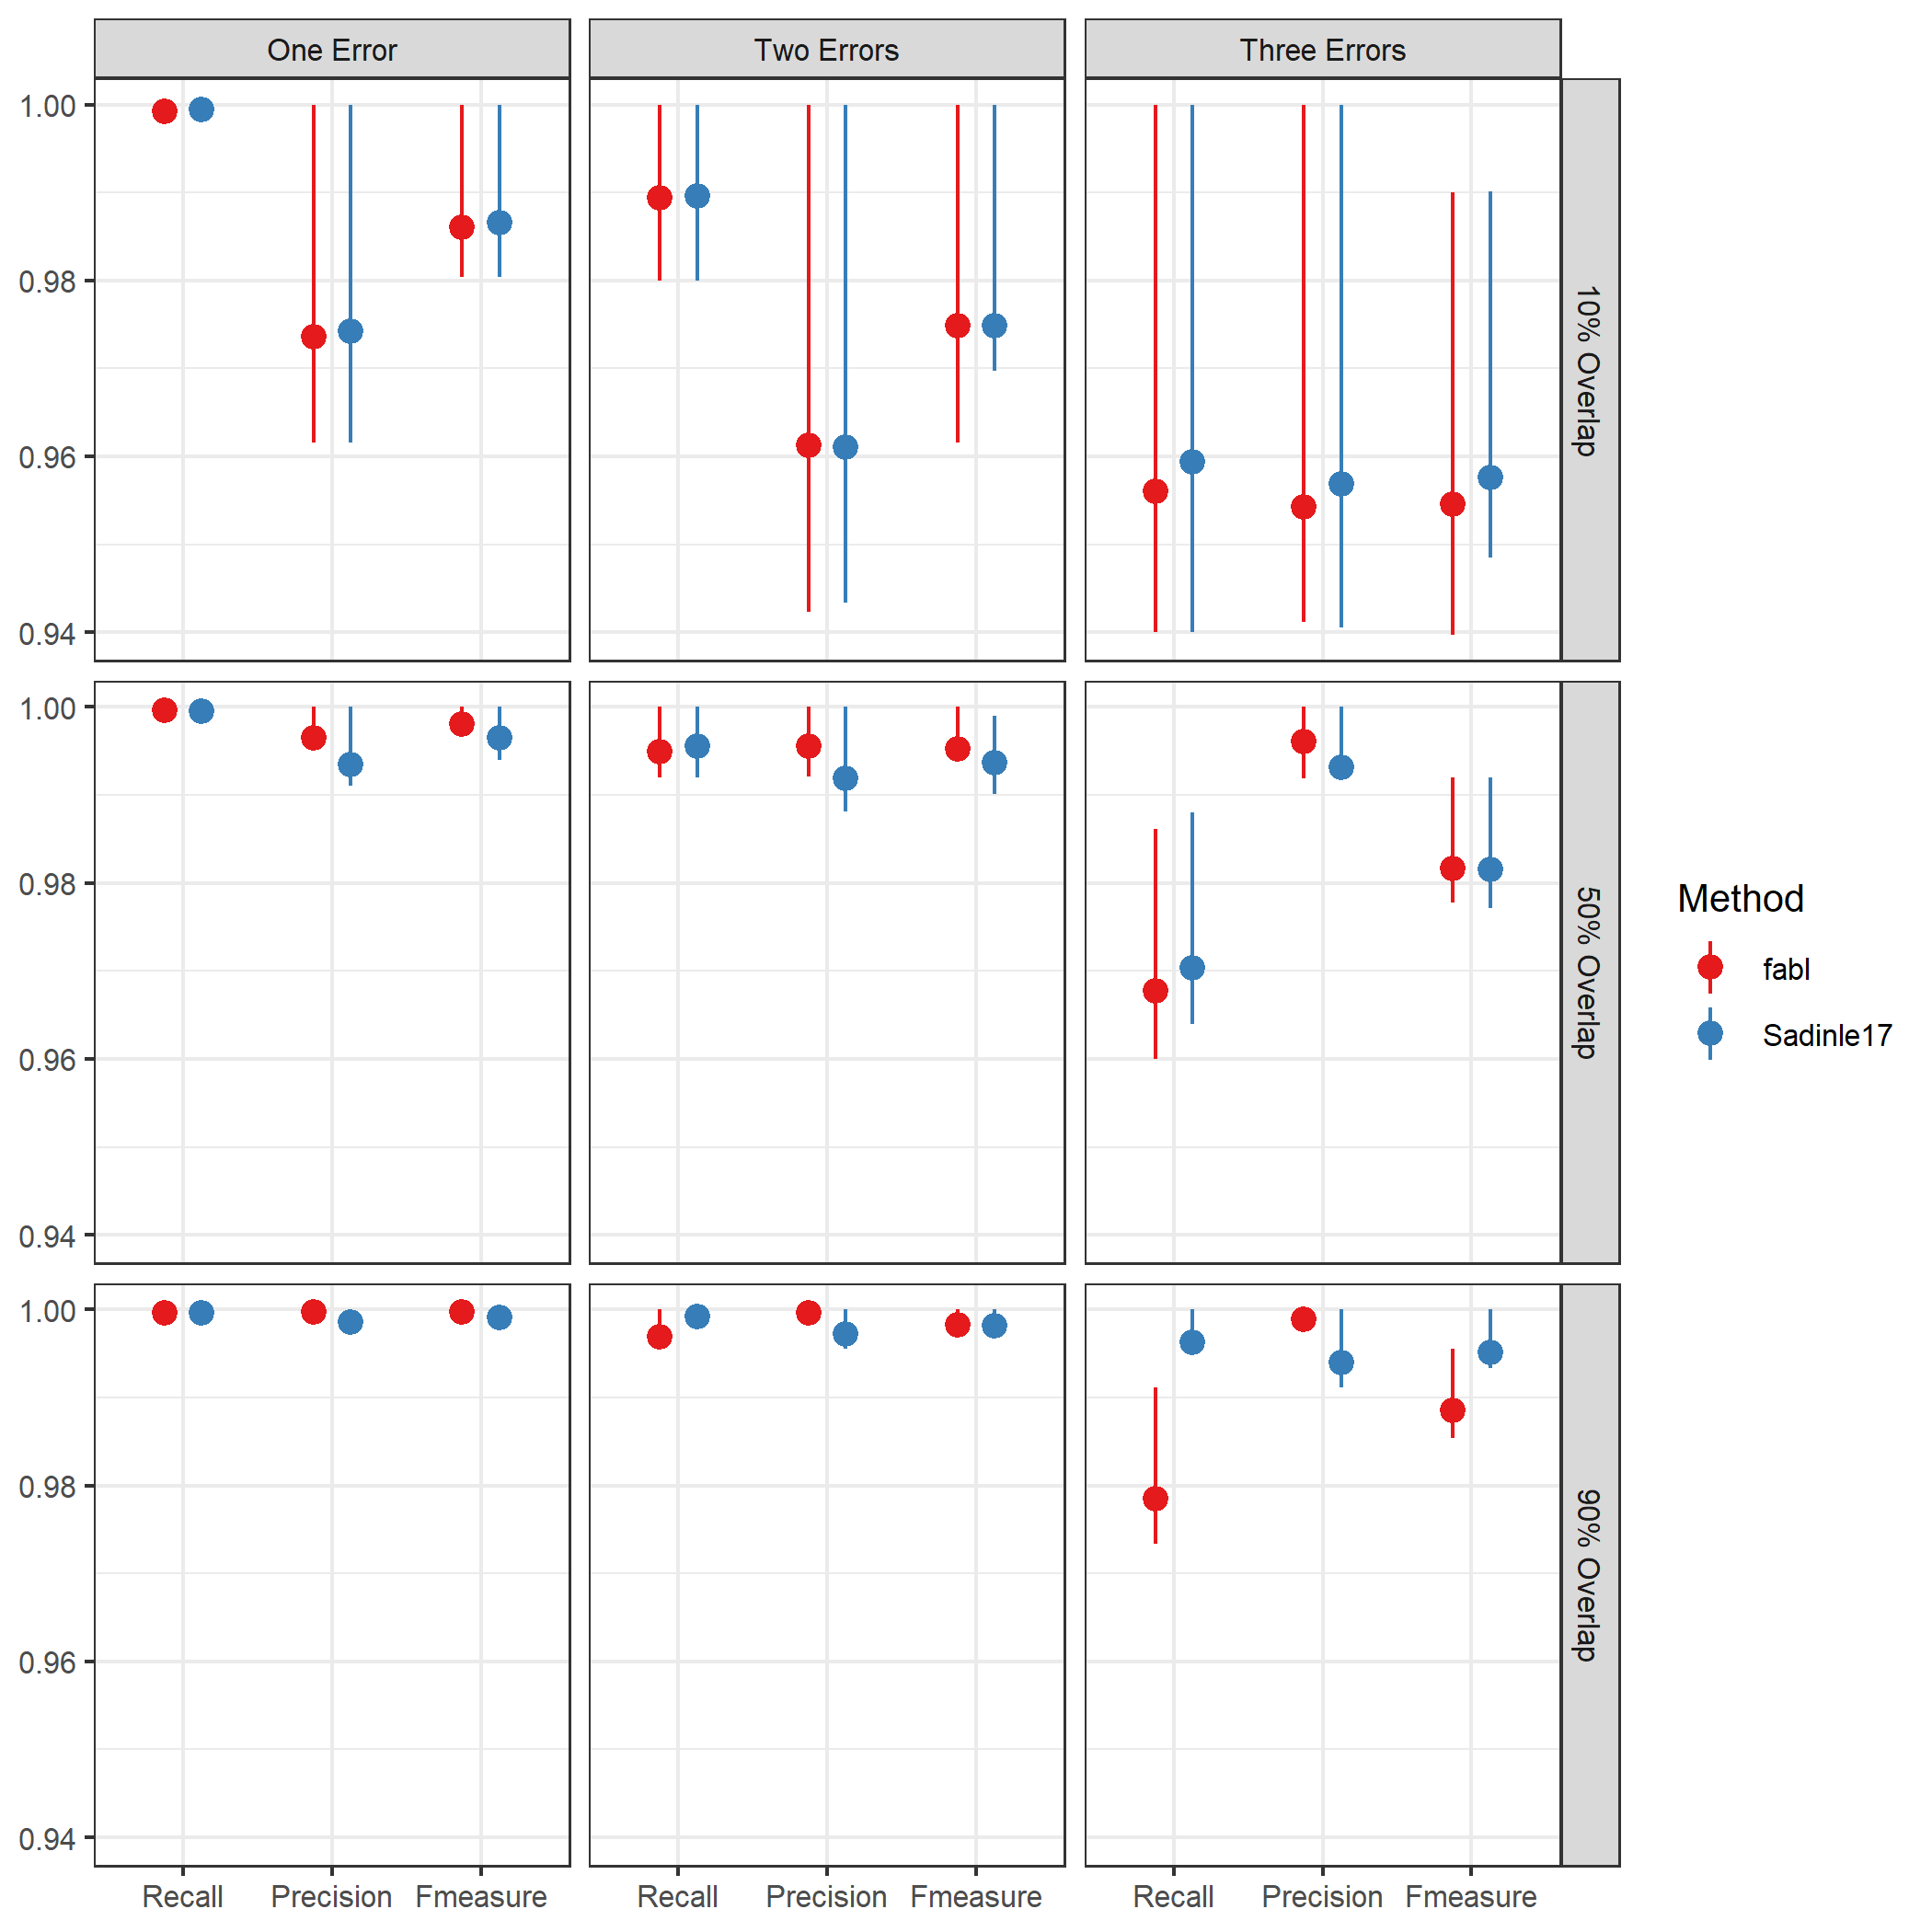
\includegraphics[width=29.17in]{../notes/figures/sadinle_sim_plot} \end{center}

\hypertarget{how-fast-is-it}{%
\subsubsection{How fast is it?}\label{how-fast-is-it}}

We simulate \(\Gamma\) matrices of comparison vectors from multinomial
distributions meant to emulate the behavior of similarity scores across
first name, last name, and day, month, and and year of birth.
Distributions provided below. We simulate these data for different
values of \(n_A and n_B\), and compare the runtime of \texttt{parlr}
against \texttt{BRL}. We note here that \texttt{BRL} is coded in C,
which makes for unfair comparison against \texttt{parlr}, currently only
built in R. We see that at low data size, \texttt{BRL} outperforms, but
that \texttt{parlr} is significantly faster at handling larger data. In
particular, runtime for \texttt{BRL} seems to grow quadratically while
runtime for \texttt{parlr} seems to grow linearly. Additionally,
although \texttt{parlr} is amenable to parallezation, this simulation
was run on a single core. Running \texttt{parlr} in C or C++ with
paralellization for the hashing step and sampling the matching status of
the record pairs should lead to even more drastic results.

\begin{center}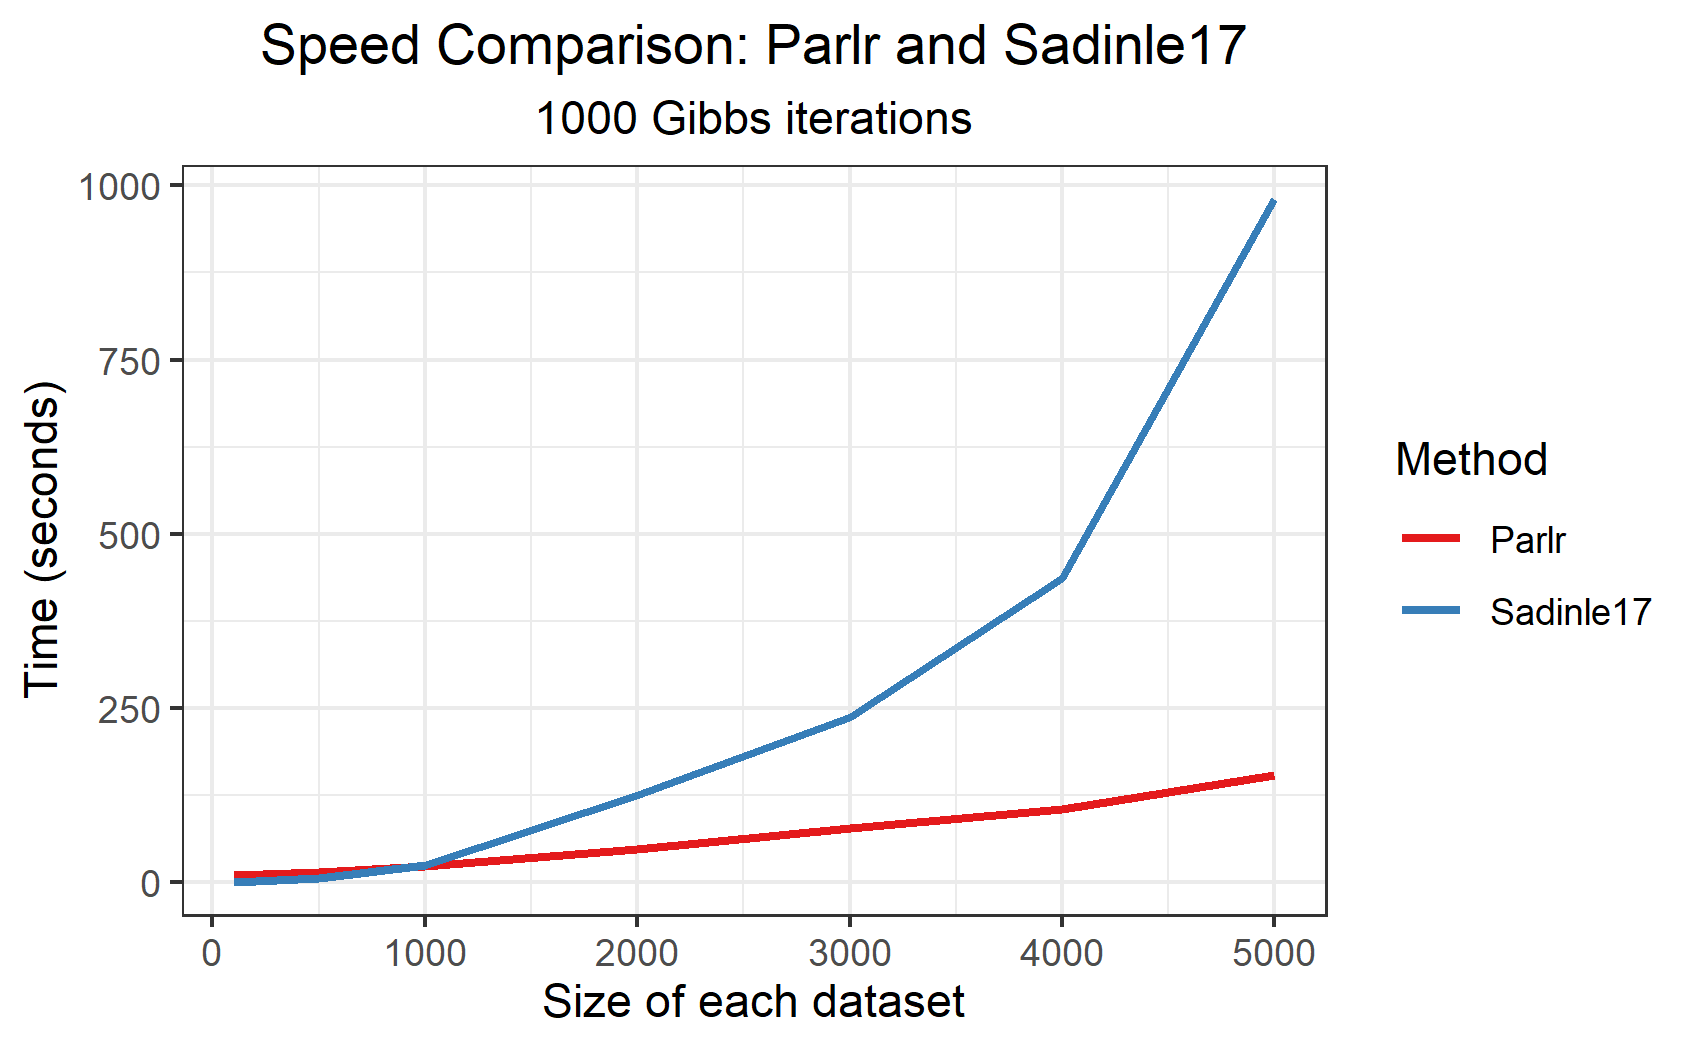
\includegraphics[width=23.6in]{../notes/figures/sadinle_speed_plot} \end{center}

The above discussion suggests that for fixed \(n_B\), computation time
should remain mostly constant with growing \(n_A\). Shockingly, this
seems to be true. In the plot below, fixing \(n_B = 500\), we see linear
growth for the runtime under \texttt{BRL} as \(n_A\) increases, with
much more static runtime under \texttt{parlr}. The slight increases in
runtime that we do see are due primarily to the hashing step, which
again can be run in parallel for large data.

\begin{center}
\includegraphics[width=29.17in]{../notes/figures/speed_plot_fixed_nB} \end{center}

\hypertarget{what-about-deduplication-of-a-single-file}{%
\subsubsection{What about deduplication of a single
file}\label{what-about-deduplication-of-a-single-file}}

At the moment, \texttt{parlr} (and its \texttt{BRL} competitor) are only
able to handle bipartite matching across two files, meaning there is
duplication across, but not within, files. Though it seems similar to
linkage across files, deduplication within one file is suprisingly much
more difficult to model probabalistically. In particular, \texttt{parlr}
assumes that the linkage decision for record \(j \in B\) is independent
from all other \(j' \in B\), allowing us to propose a prior
\(\lambda \sim \text{Beta}(\alpha, \beta)\) for the probability of \(j\)
having some match in \(A\), and update that prior through standard
beta-binomial posterior updates. With only one file however, if the
sampler decides that record \(1\) matches with record \(5\), there is no
way to determine the linkage of record \(5\) independently; we do not
even have \(n_B\) independent linkage decisions to work with!
Constructing fast, scalable methods for deduplication is one avenue of
future work.

\hypertarget{anything-else}{%
\subsubsection{Anything else?}\label{anything-else}}

Kundinger is particularly interested in linkage scenarios when the
reliability of the data (the level of error in the fields), and the
rates of matching, differ by subgroups in the data. The simplest case of
this occurs when matching historical records for women; due to marriage
conventions, the last name is a much less reliable identifier for women
than for men. In an upcoming extention, we propose \emph{linkage
clusters} that account these difficulties, while still maintaining the
computational advances from \texttt{parlr}.

\end{document}
